
%Electrically charged particles, such as electrons, quarks, and the $W^{\pm}$ bosons, to name a few, interact via 
The Electromagnetic (EM) interaction is described in the SM by an Abelian gauge theory called Quantum Electrodynamics (QED) with the gauge group \Uone. The \Uone symmetry allows a gauge transformation of the EM vector field $A^{\mu}$ to be made:
\begin{equation}
    A^{\mu} \rightarrow A'^{\mu} = A^{\mu} + \partial^{\mu}\chi
\end{equation}
with no change to the free-field lagrangian. Allowing the EM field to couple to (interact with) electrically charged Dirac fermions $\psi$, while imposing invariance on the whole QED lagrangian (free field + interacting terms), requires a simultaneous (and local) phase transformation of $\psi$:
\begin{equation}
    \psi \rightarrow \psi' = e^{-ie\chi(x)}\psi
\end{equation}
with the factor $e$ on the phase being the experimentally measured charge of the electron (related to the coupling strength of $A^{\mu}$ to $\psi$). These gauge transformations forbid any mass and self-interacting terms of $A^{\mu}$ from appearing in the QED lagrangian, and restrict the quanta of $A^{\mu}$ to vector bosons. Photons are consistent with the constraints of the \Uone~symmetry of QED (being massless spin 1 bosons that do not self-interact) and were confirmation that QED was an accurate description of the EM force. As with the other two forces in the SM, we say that the photon ``mediates'' EM interactions between particles charged under QED, as the photon's coupling to electrically charged particles is responsible for the forces between them. For example, the Feynman diagram in Fig.~\ref{fig:QEDFeynmanDiagram} shows the electromagnetic repulsion of two electrons propogating through space-time by the exchange of a virtual photon, the mediator of the EM force. 
\begin{figure}[H]
    \centering
    \vspace{0.05\textwidth}
    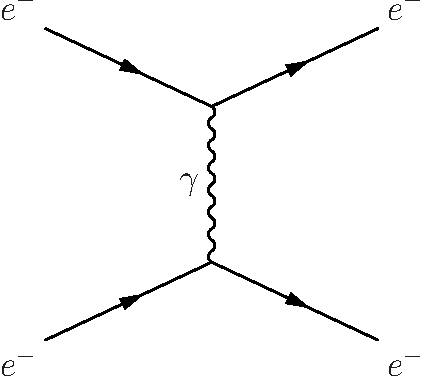
\includegraphics[width=0.3\textwidth]{Images/QEDInteraction.pdf}\hspace{0.1\textwidth}
    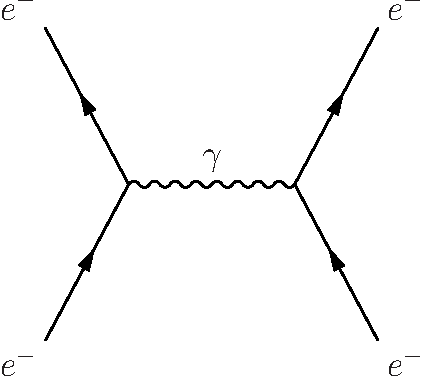
\includegraphics[width=0.3\textwidth]{Images/QED_s_channel.pdf}\vspace{0.05\textwidth}
    \caption{Left: A tree-level Feynman diagram in the $t$-channel showing two electrons interacting (repelling) via the exchange of a virtual photon. Right: Rotating the $t$-channel diagram 90 degrees gives the $s$-channel diagram, showing the annihilation of an electron-antielectron pair into a virtual photon, which propagtes before decaying again into an electron-antielectron pair. Both phenomena are described with QED.}
    \label{fig:QEDFeynmanDiagram}
\end{figure}
At very high energies (such as shortly after the big bang) the EM interaction is understood to be unified with the weak interaction, collectively called the electroweak force, that is only broken into separate forces at a temperature of approximately $10^{15}$~K (explained in more detail in Section~\ref{sec:WeakInteraction}).